\documentclass[11pt,a4paper]{article}
\usepackage[margin=0.82in]{geometry}
\usepackage[T1]{fontenc}
\usepackage{lmodern}
\usepackage{amsmath,amssymb}
\usepackage{graphicx}
\usepackage{float}
\usepackage{microtype}
\usepackage[hidelinks]{hyperref}
\emergencystretch=3em

\newcommand{\Mloc}{M_{\mathrm{loc}}}

\title{The Local-Multiplier Idempotence Question\\[0.3em]
\large A negative answer in arXiv:math/0509437}
\author{Automated Mathematics Run \texttt{fa\_banach\_001}, lane 0}
\date{13 August 2026}

\begin{document}
\sloppy
\hbadness=2000
\maketitle

\begin{center}
\fbox{\parbox{0.92\linewidth}{\textbf{Status: literature already answered
(negative).} No new theorem is claimed. Ara and Mathieu construct unital,
primitive AF algebras whose second local multiplier algebra is strictly larger
than the first, refuting the universal equality stated in Frank--Paulsen.}}
\end{center}

\section{The source question}

For a $C^*$-algebra $A$, let $\Mloc(A)$ denote its local multiplier algebra.
Frank and Paulsen~\cite{FP} state on page 15 that one of the main open
questions in the theory is whether
\begin{equation}\label{eq:question}
  \Mloc(A)=\Mloc(\Mloc(A))
\end{equation}
for every $C^*$-algebra $A$.

\begin{figure}[H]
  \centering
  
\includegraphics[width=0.92\linewidth]{figures/source_question_crop.png}
  \caption{Frank--Paulsen, arXiv:math/0106131, PDF page 15.}
\end{figure}

Their subsequent theorem places every iterated local multiplier algebra inside
the same injective envelope, but it does not prove equality in
\eqref{eq:question}.

\section{The later counterexample}

Ara and Mathieu~\cite{AM} revisit the same equality. Their abstract says they
construct an AF algebra for which the two local multiplier algebras do not
agree, thereby answering the question raised by Pedersen. In the introduction
they label \eqref{eq:question} as Question (2), explicitly say that its answer
is negative, and state:

\begin{center}
\fbox{\parbox{0.82\linewidth}{\textbf{Theorem 1.1 (Ara--Mathieu).}
There exist unital, primitive AF algebras $A$ such that
\[
 \Mloc(\Mloc(A))\ne\Mloc(A).
\]}}
\end{center}

\begin{figure}[H]
  \centering
  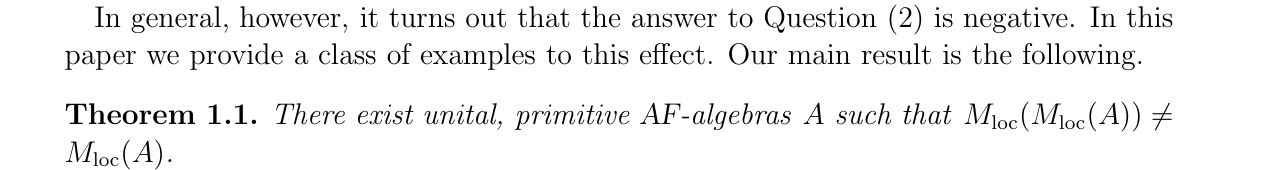
\includegraphics[width=0.94\linewidth]{figures/supporting_theorem_crop.png}
  \caption{Ara--Mathieu, arXiv:math/0509437, PDF page 2.}
\end{figure}

This is a literal counterexample to the universal quantifier in
\eqref{eq:question}.  The answer is therefore complete and negative, already
in the restrictive class of unital primitive AF algebras.

\section{Provenance, scope, and verification}

The local registry and attempt indexes contained no prior row for
arXiv:math/0106131. A bounded exact-formula and keyword search located
arXiv:math/0509437 and the later survey arXiv:1110.6858, which confirms that
several such examples are now known. The displayed question and theorem were
then checked directly in the two primary PDFs included in this packet.

The other source signals---classification of relatively injective
$C^*$-algebras and characterization of algebras satisfying
$\Mloc(A)=I(A)$---are broader programs and are not claimed to be resolved by
the cited counterexample. This packet clears only the exact iterated-local-
multiplier equality.

\begin{thebibliography}{9}
\bibitem{FP}
M.~Frank and V.~I.~Paulsen,
\emph{Injective Envelopes of $C^*$-algebras as Operator Modules},
arXiv:math/0106131.

\bibitem{AM}
P.~Ara and M.~Mathieu,
\emph{A not so simple local multiplier algebra},
arXiv:math/0509437 (2005).
\end{thebibliography}

\end{document}
